%\newcommand{\novathesis}{\emph{novathesis}}
%\newcommand{\novathesisclass}{\texttt{novathesis.cls}}

\chapter{Development}
\label{development}

\section{Requirements and properties}
\label{req}

Materials requirements are defined in standard MEP 15-047 for the ATL material, table \ref{table:atlmaterialreq} and MEP 15-067 for the AFP material, table \ref{table:afpmaterialreq}.

% Please add the following required packages to your document preamble:
% \usepackage{booktabs}
% \usepackage{multirow}
\begin{table}[htbp]
\centering
\setlength\aboverulesep{0pt}\setlength\belowrulesep{0pt}
\caption{Physical and Mechanical Requirements for ATL material}
\label{table:atlmaterialreq}
\resizebox{\textwidth}{!}{%
\begin{tabular}{@{}ccccc@{}}
\toprule
\multicolumn{5}{c}{\textbf{Mechanical Requirements}}                                                                                                                                                                                                                                                                              \\ \midrule
\multicolumn{1}{c|}{\multirow{2}{*}{\textbf{Property}}}                      & \multicolumn{1}{c|}{\multirow{2}{*}{\textbf{Test temperature and environmental condition}}} & \multicolumn{2}{c|}{\textbf{Stregth Requirement {[}MPa{]}}}                                & \multirow{2}{*}{\textbf{Modulus Requirement {[}GPa{]}}} \\ \cmidrule(lr){3-4}
\multicolumn{1}{c|}{}                                                        & \multicolumn{1}{c|}{}                                                                       & \multicolumn{1}{l|}{\textbf{Min. Average}} & \multicolumn{1}{l|}{\textbf{Min. Individual}} &                                                         \\ \midrule
\multicolumn{1}{c|}{\multirow{2}{*}{\textbf{Interlaminar 0º Direction}}}     & \multicolumn{1}{c|}{RTA}                                                                    & \multicolumn{1}{c|}{103}                   & \multicolumn{1}{c|}{96}                       & N.A.                                                    \\ \cmidrule(l){2-5} 
\multicolumn{1}{c|}{}                                                        & \multicolumn{1}{c|}{ETW}                                                                    & \multicolumn{1}{c|}{63}                    & \multicolumn{1}{c|}{59}                       & N.A.                                                    \\ \midrule
\multicolumn{1}{c|}{\multirow{2}{*}{\textbf{Interlaminar Tension Strength}}} & \multicolumn{1}{c|}{RTA}                                                                    & \multicolumn{1}{c|}{TBD}                   & \multicolumn{1}{c|}{TBD}                      & TBD                                                     \\ \cmidrule(l){2-5} 
\multicolumn{1}{c|}{}                                                        & \multicolumn{1}{c|}{ETW}                                                                    & \multicolumn{1}{c|}{TBD}                   & \multicolumn{1}{c|}{TBD}                      & TBD                                                     \\ \midrule
\multicolumn{5}{c}{\textbf{Physical Requirements}}                                                                                                                                                                                                                                                                                \\ \midrule
\multicolumn{2}{c|}{\textbf{Property}}                                                                                                                                     & \multicolumn{2}{c|}{\textbf{Requirement}}                                                  & \textbf{Unit}                                           \\ \midrule
\multicolumn{2}{c|}{\textbf{Laminate Thickness per Ply}}                                                                                                                   & \multicolumn{2}{c|}{0,184 $\pm$ 0,020}                                                     & {[}mm{]}                                                \\ \midrule
\multicolumn{2}{c|}{\textbf{Fourier Tranform Infrared (FTIR)}}                                                                                                             & \multicolumn{2}{c|}{Informative}                                                           & N.A.                                                    \\ \midrule
\multicolumn{2}{c|}{\textbf{Differential Scanning Calorimetry (DSC)}}                                                                                                      & \multicolumn{2}{c|}{Informative}                                                           & N.A.                                                    \\ \midrule
\multicolumn{2}{c}{\textbf{Differencial Mechanical Analysis (DMA)}}                                                                                                        & \multicolumn{2}{c}{T$_g$(dry)  = 210}                                                      & {[}ºC{]}                                                \\ \bottomrule
\end{tabular}
}
\end{table}

% Please add the following required packages to your document preamble:
% \usepackage{booktabs}
% \usepackage{multirow}
\begin{table}[htbp]
\centering
\setlength\aboverulesep{0pt}\setlength\belowrulesep{0pt}
\caption{Physical and Mechanical Requirements for AFP material}
\label{table:afpmaterialreq}
\resizebox{\textwidth}{!}{%
\begin{tabular}{@{}ccccc@{}}
\toprule
\multicolumn{5}{c}{\textbf{Mechanical Requirements}}                                                                                                                                                                                                                                                                              \\ \midrule
\multicolumn{1}{c|}{\multirow{2}{*}{\textbf{Property}}}                      & \multicolumn{1}{c|}{\multirow{2}{*}{\textbf{Test temperature and environmental condition}}} & \multicolumn{2}{c|}{\textbf{Stregth Requirement {[}MPa{]}}}                                & \multirow{2}{*}{\textbf{Modulus Requirement {[}GPa{]}}} \\ \cmidrule(lr){3-4}
\multicolumn{1}{c|}{}                                                        & \multicolumn{1}{c|}{}                                                                       & \multicolumn{1}{l|}{\textbf{Min. Average}} & \multicolumn{1}{l|}{\textbf{Min. Individual}} &                                                         \\ \midrule
\multicolumn{1}{c|}{\multirow{2}{*}{\textbf{Interlaminar 0º Direction}}}     & \multicolumn{1}{c|}{RTA}                                                                    & \multicolumn{1}{c|}{88,1 (13)}             & \multicolumn{1}{c|}{77,2 (11)}                & N.A.                                                    \\ \cmidrule(l){2-5} 
\multicolumn{1}{c|}{}                                                        & \multicolumn{1}{c|}{ETW}                                                                    & \multicolumn{1}{c|}{60,1 (9)}              & \multicolumn{1}{c|}{52,6 (8)}                 & N.A.                                                    \\ \midrule
\multicolumn{1}{c|}{\multirow{2}{*}{\textbf{Interlaminar Tension Strength}}} & \multicolumn{1}{c|}{RTA}                                                                    & \multicolumn{1}{c|}{TBD}                   & \multicolumn{1}{c|}{TBD}                      & TBD                                                     \\ \cmidrule(l){2-5} 
\multicolumn{1}{c|}{}                                                        & \multicolumn{1}{c|}{ETW}                                                                    & \multicolumn{1}{c|}{TBD}                   & \multicolumn{1}{c|}{TBD}                      & TBD                                                     \\ \midrule
\multicolumn{5}{c}{\textbf{Physical Requirements}}                                                                                                                                                                                                                                                                                \\ \midrule
\multicolumn{2}{c|}{\textbf{Property}}                                                                                                                                     & \multicolumn{2}{c|}{\textbf{Requirement}}                                                  & \textbf{Unit}                                           \\ \midrule
\multicolumn{2}{c|}{\textbf{Laminate Thickness per Ply}}                                                                                                                   & \multicolumn{2}{c|}{0,191 $\pm$ 0,010}                                                     & {[}mm{]}                                                \\ \midrule
\multicolumn{2}{c|}{\textbf{Fourier Tranform Infrared (FTIR)}}                                                                                                             & \multicolumn{2}{c|}{Informative}                                                           & N.A.                                                    \\ \midrule
\multicolumn{2}{c|}{\textbf{Differential Scanning Calorimetry (DSC)}}                                                                                                      & \multicolumn{2}{c|}{Informative}                                                           & N.A.                                                    \\ \midrule
\multicolumn{2}{c}{\textbf{Differencial Mechanical Analysis (DMA)}}                                                                                                        & \multicolumn{2}{c}{T$_g$(dry)  = {[}210;230{]}}                                            & {[}ºC{]}                                                \\ \bottomrule
\end{tabular}
}
\end{table}
 
\section{Testing}
\label{tests}

\subsection{Testing conditions}
\label{testingc}

Test condition will be at \gls{rta}, described below. Other testing conditions are advised, but due to time constraints it was not possible to arrange such testing conditions.

\begin{itemize}
\item \textbf{RTA} - Temperature at 23ºC $\pm$ 3ºC, with specimens conditioned in Ambient conditioning as ASTM D618/procedure A:
	\begin{itemize}
		\item Condition 40/23/50 for specimens 7 mm or under in thickness - condition test specimens 7 mm or under in thickness in the standard laboratory atmosphere for a minimum of 40 hours immediately prior to testing. Provide adequate air circulation on all sides of the test.
	\end{itemize}
\end{itemize}

\subsection{Physical testing}
\label{sec:physical}

Due to the nature of the prepreg, most physical testing will focus on uncured prepreg. These test will help us assess the material properties before and after the co-cure provided by hot forming thermal cycle. Each one of this physical tests are intended to a specific function, according its results and functioning. However, Ply thickness is measured in cured laminates. Although it is not a prepreg test, it is a measure of a physical property, therefore will be considered a physical test.

\begin{itemize}
	\item Ply thickness;
	\item \gls{ftir};
	\item \gls{dsc};
	\item \gls{dma}.
\end{itemize}

\subsection{Mechanical testing}
\label{sub:mechanical}

Mechanical testing is needed to aid the scope of this thesis: Evaluate the prepreg after hot drape thermal cycle and exposure conditions. These tests will be the ones to give us the mechanical properties after the co-cure. It'll be important to assess the effects of the thermal cycle, together with material exposure. 

\begin{itemize}
	\item \texorpdfstring{\gls{ils}};
	\item \gls{ilts}.
\end{itemize}


\section{Material exposure conditions}
\label{expcond}

The material exposure conditions are expressed in table \ref{materialconditions}. In order to optimize production, conditions 1 to 4 will be laminated in bulk, except for the 'L' shaped mold. Condition 5 requires a more complicated aging, with revalidation tests to assure material quality. 

\begin{table}[htbp]
\centering
\caption{Material exposure conditions}
\label{materialconditions}
\resizebox{\textwidth}{!}{
	\begin{threeparttable}
		\begin{tabular}{c|cccc}
			Condition          & Material Out Time        & Hot Drape            & Additional Out Time After Hot Drape & Cure                            \\ \hline
			1                  & Minimum \tnote{1}        & No                   & No                                  & After lamination                \\
			2                  & Minimum \tnote{1}        & Yes                  & No                                  & After hot drape                 \\
			3                  & Maximum \tnote{2}        & Yes                  & No                                  & After hot drape                 \\
			\multirow{2}{*}{4} & 10 days for ATL material & \multirow{2}{*}{Yes} & \multirow{2}{*}{Maximum \tnote{2}}  & \multirow{2}{*}{Out time limit} \\
			                   & 11 days for AFP material &                      &                                     &                                 \\
			5                  & Revalidated +200h        & Yes                  & No                                  & After hot drape                
		\end{tabular}

		\begin{tablenotes}	
			\item[1] 2 days of accumulated out time allowed
			\item[2] 2 days of available of out time allowed
		\end{tablenotes}
	\end{threeparttable}
}
\end{table}

\section{Fabrication}
\label{testfabrication}

While sorting material to use for experimentation, shelf life was highly regarded. Out time had a special importance in selecting tows for AFP, since there was a high volume of material within our exposure conditions. Hence aging was mostly for condition 4 and 5, regarding AFP material. After material selection, material would unfreeze for 8 hours at least. In some cases, different batches were used in producing the same panel. Out time condition was regarded higher than batch uniformity, since this would save material.


Material selection - Roll number, batch, exposure.

Vacuum bag

Lamination programs

Lamination problems

\subsection{Panels and specimens}
\label{panels}

Panel fabrication was planned regarding the tests needed and which requirements were needed to meet. Considering the fact that two mechanical tests were intended, two panels were to be manufactured. One regarding ILSS test, which were used to DMA as well, and one regarding ILTS. As both have to fulfill material exposure conditions detailed in section \ref{materialconditions}, a panel would needed to be manufactured for each condition. Therefore, a total of 20 panels were created.

For each panel, intended sample size was of 15 specimen. However, because of some constraints regarding panel quality mentioned in section \ref{testfabrication}, some panels sample size were reduced. 

\subsubsection{Specimen nomenclature}
\label{nomenclature}

In order to facilitate specimen identification and testing, specimens were identified using the following nomenclature:

\begin{figure}[htbp]
\setlength{\belowcaptionskip}{-10pt}
\label{img:naming}
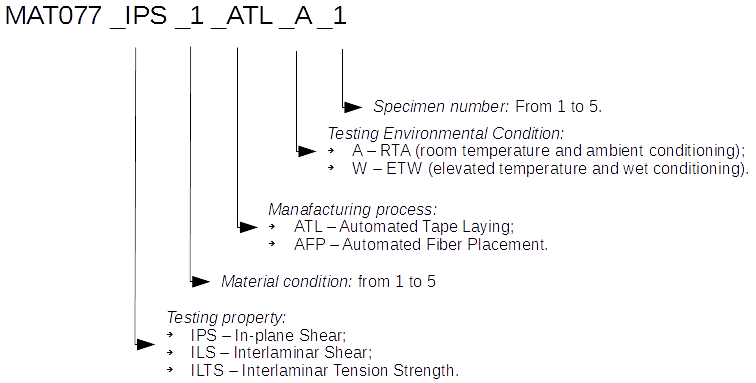
\includegraphics[width=\textwidth]{Chapters/Figures/naming.png}
\caption{Specimen naming code.}
\end{figure}
